\section{Methodology}
\label{sec:methodology}
Our approach combines multiple techniques to create efficient and compact embeddings while preserving semantic relationships. The key components include:
\begin{itemize}
    \item Neural transformation layers for improved quantization and matryoshka representation learning
    \item Hybrid architecture combining different quantization levels
    \item Loss functions to promote quantization and matryoshka representation learning
    \item Efficient bit-packing and similarity computation
\end{itemize}

\begin{figure*}[h]
    \centering
    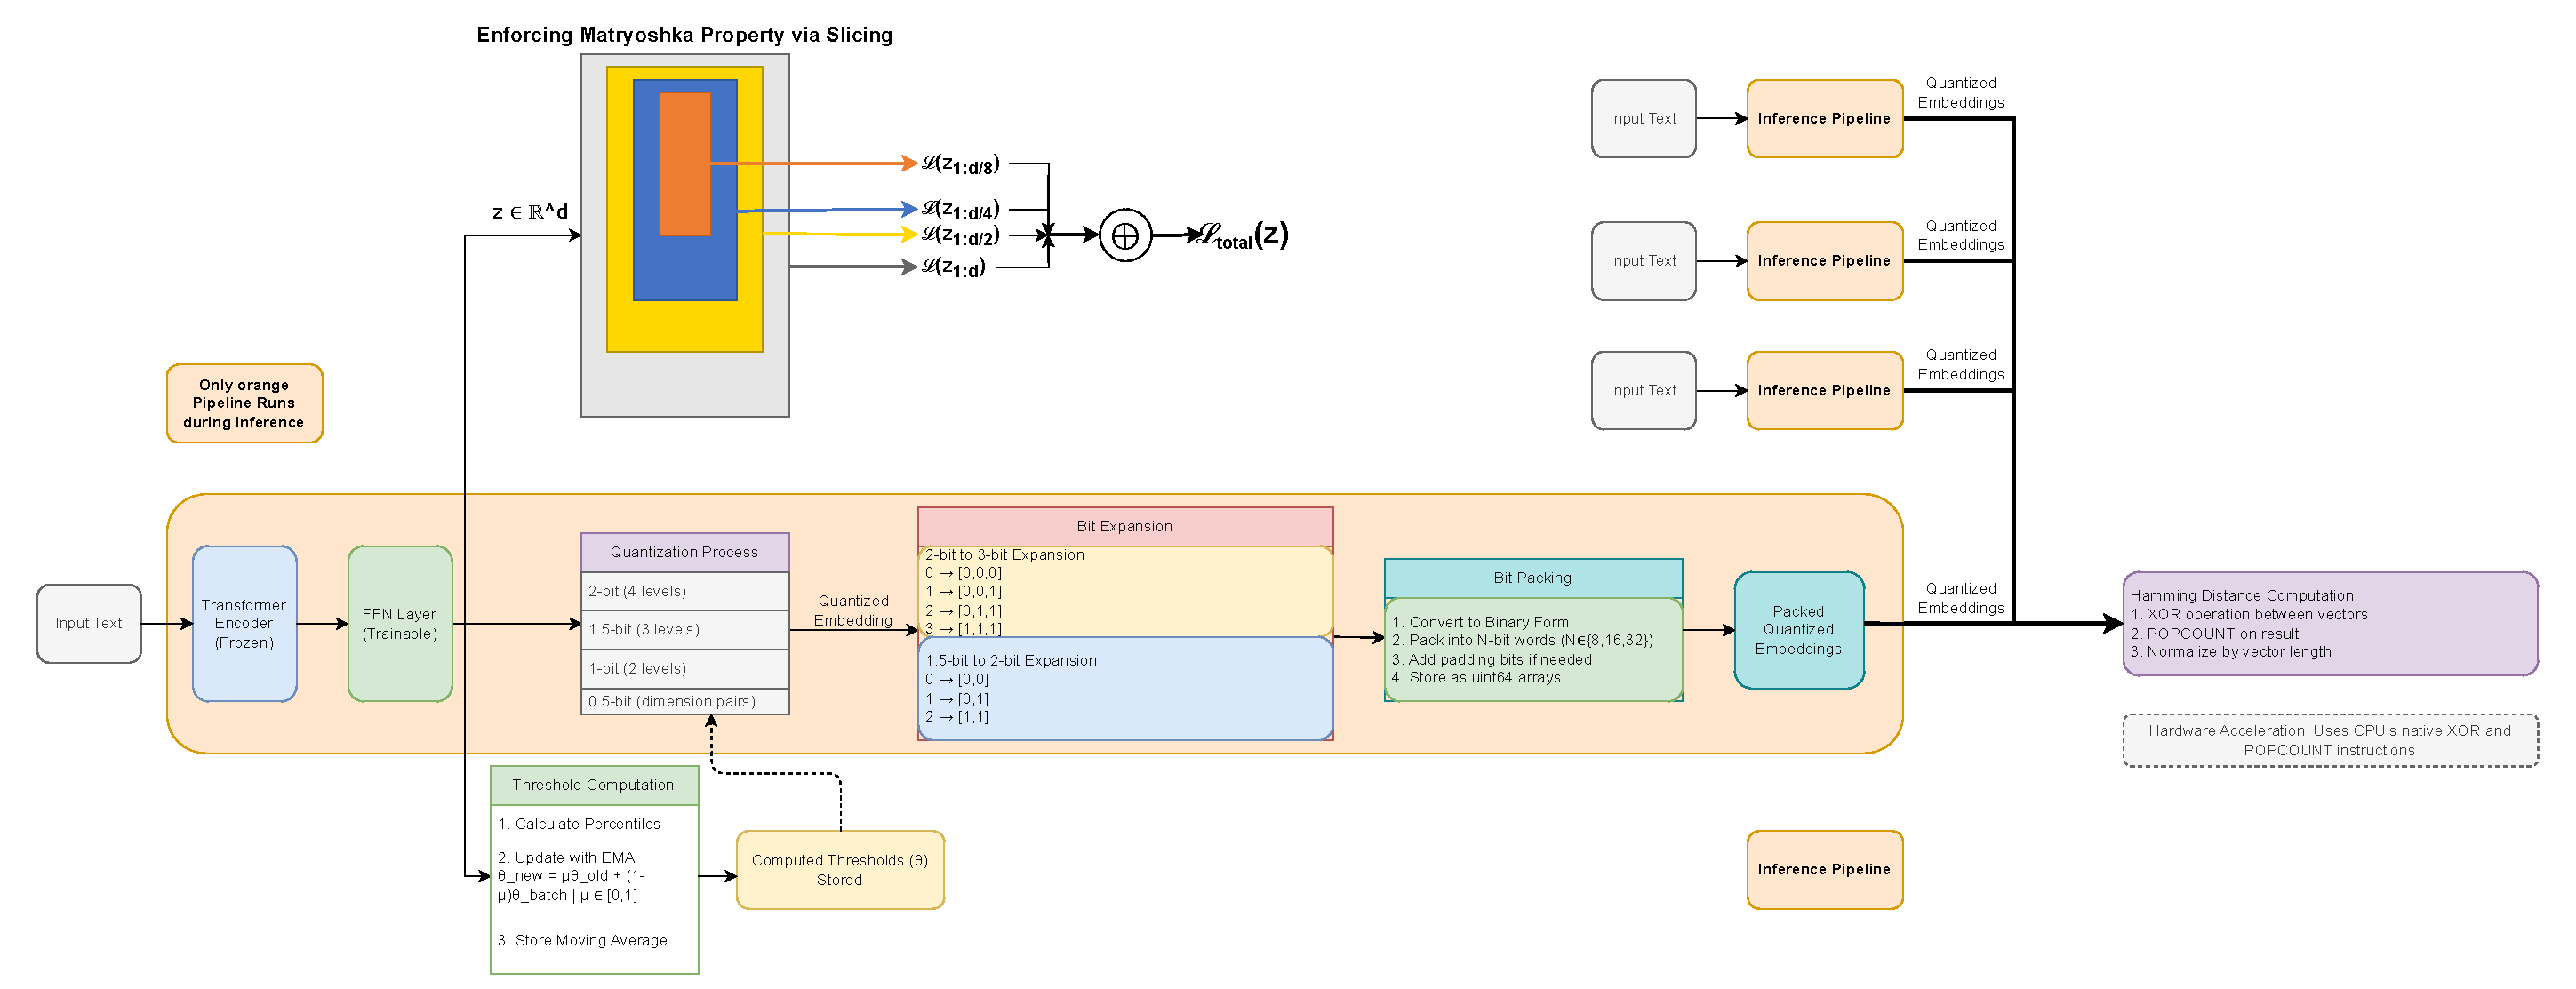
\includegraphics[width=\textwidth]{main-diagram.pdf}
    \caption{Overall architecture of QAMA system showing the transformation, quantization, and bit-packing stages.}
    \label{fig:system_architecture}
\end{figure*}


\subsection{Quantization Framework}
\label{subsec:quantization_framework}

Our quantization framework converts high-precision embeddings into compact, discrete representations while preserving semantic relationships through a combination of neural transformations and adaptive threshold-based discretization. We first apply a feedforward transformation $\mathbf{z} = \text{FFN}(\mathbf{x}; \theta)$ to optimize the embedding space for quantization, where $\mathbf{x}$ is the input embedding and $\theta$ represents trainable parameters.
We implement multiple quantization levels for flexible storage-performance trade-offs: 2-bit (4 levels), 1.5-bit (3 levels), 1-bit (2 levels), and 0.5-bit (combines dimension pairs) quantization. For $k$-bit quantization with $2^k$ levels, we use $(2^k - 1)$ learnable thresholds per dimension to partition the continuous embedding space. For instance, 2-bit quantization employs three thresholds $\{\theta_1, \theta_2, \theta_3\}$ to create four bins, while 1-bit quantization uses a single threshold for binary partitioning.
For a $d$-dimensional embedding space $\mathbf{X} \in \mathbb{R}^{N \times d}$, we initialize thresholds using percentile statistics to ensure balanced quantization: $\theta_{i,j} = \text{Quantile}\bigl(\{x_{1,j}, \ldots, x_{N,j}\},\; q_i\bigr)$
where $q_i$ are evenly-spaced quantiles in $(0,1)$. During training, thresholds adapt via exponential moving average: $$\theta_{i,j}^{(\text{new})} = \mu\,\theta_{i,j}^{(\text{old})} + (1-\mu)\;\widehat{\theta}_{i,j}^{(\text{batch})}$$
with momentum coefficient $\mu \in [0,1]$ and batch-computed thresholds $\widehat{\theta}_{i,j}^{(\text{batch})}$.
The complete process for an input embedding involves: (1) applying the trainable transformation $\mathbf{z} = \text{FFN}(\mathbf{x})$, (2) normalizing $\hat{\mathbf{z}} = \text{normalize}(\mathbf{z})$, and (3) assigning discrete codes: $q_j = \sum_{i=1}^{2^k-1} \mathbbm{1}[\hat{z}_j > \theta_{i,j}]$

\paragraph{End-to-End Trainability}
Our framework achieves end-to-end trainability by optimizing continuous-valued embeddings while simultaneously guiding them toward quantization-friendly distributions. 
Rather than backpropagating through non-differentiable quantization operations, we apply quantization regularization losses (Section~\ref{subsubsec:quant_reg}) that encourage embeddings to cluster away from quantization boundaries. 
The thresholds themselves are updated using statistics from the continuous embeddings.%, ensuring the quantization boundaries evolve to match the learned representation space, while the transformation network learns to produce embeddings that naturally align with discrete quantization levels, enabling training without direct gradients through the discretization step.
% This framework offers several advantages: optimal organization of embedding dimensions through learned transformations, balanced quantization bins via adaptive thresholds, flexible storage-performance trade-offs through multiple quantization levels, and end-to-end trainability. 
% Experimental results (Section~\ref{sec:experiments}) demonstrate significant compression while maintaining high retrieval accuracy across diverse tasks.


\subsection{Promoting Information High Density in Early Dimensions}
\label{subsec:matryoshka_and_control}
Matryoshka Representation Learning (MRL) creates embeddings that maintain effectiveness when truncated. Unlike traditional embeddings where key features span all dimensions, our enhanced MRL approach concentrates critical information in early dimensions through controlled nesting.
% Matryoshka Representation Learning (MRL), addresses a fundamental challenge in embedding systems: creating representations that remain effective when truncated to smaller dimensions. 
% Traditional embeddings often lose critical information when dimensions are removed since important features are distributed across all dimensions. 
% Our approach extends MRL with additional control mechanisms to create highly efficient, nested representations where the most crucial information is concentrated in early dimensions.
% inspired by Russian nesting dolls,
% \subsubsection{Core Matryoshka Architecture}
\paragraph{Nested Representation Generation}
Given an input embedding $\mathbf{x} \in \mathbb{R}^d$, we generate a series of nested representations at different dimension levels $\mathcal{D} = \{d_1, d_2, ..., d_K\}$ where $d_1 < d_2 < ... < d_K = d$. 
First, we transform the input through a feed-forward network: $\mathbf{z} = \text{FFN}(\mathbf{x}; \theta) \in \mathbb{R}^d$

Unlike traditional MRL implementations that use separate projections for each scale, we employ an efficient progressive slicing mechanism.
We create level-specific representations through progressive slicing:
\begin{equation}
    \mathbf{z}_k = \text{Slice}_{d_{k-1}}^{d_k}(\mathbf{z}), \quad k = 1,\ldots,K
\end{equation}

The key nesting property ensures that smaller representations are perfect subsets of larger ones: $\mathbf{z}_i[1:d_j] = \mathbf{z}_j \quad \text{for } j < i$
The full embedding at level $k$ is constructed through concatenation: $\mathbf{e}_k = [\mathbf{z}_1; \mathbf{z}_2; ...; \mathbf{z}_k]$
We implement the transformation function $\text{FFN}$ using the same lightweight yet effective feed-forward network as introduced in the quantization framework, where $\mathbf{z} = \text{FFN}(\mathbf{x}; \theta) = \mathbf{W}_2(\text{GELU}(\mathbf{W}_1\mathbf{x}))$. 
This approach inherently maintains the nested property without requiring explicit constraints, reducing computational overhead.

\paragraph{Combined Loss Function}
Our training objective combines multiple loss components, each with their corresponding weights, applied at each dimension level:

\begin{equation}
\begin{split}
    \mathcal{L}_{\text{total}} = & \sum_{d \in \mathcal{D}} \sum_{l \in \mathcal{L}} w_l^{(d)} \mathcal{L}_l^{(d)}
\end{split}
\end{equation}

where $w_l^{(d)}$ represents the weight for loss component $l$ at dimension level $d$.
\subsection{Loss Functions and Training Objectives}
\label{subsec:loss_functions}

In our proposed Matryoshka Representation Learning (MRL) framework, we integrate both \emph{similarity preservation} and \emph{matryoshka adaptation} losses to achieve nested, multilevel embeddings that maintain semantic quality at each quantization level.
Additionally, a \emph{quantization regularization} component ensures that the learned representation is readily quantizable with minimal loss in accuracy. 
% Below, we detail each category of losses and explain how they contribute to our overall training scheme.

\subsubsection{Similarity Preservation}
\paragraph{Direct Similarity MSE Loss}
We first ensure preservation of pairwise similarities via a mean squared error (MSE) loss on the normalized similarity matrices:
\begin{equation}
    \mathcal{L}_{\text{sim}}(\mathbf{X}, \mathbf{Y}) = \|\mathbf{S}_X - \mathbf{S}_Y\|_F^2
\end{equation}
where $\mathbf{S}_X = \text{normalize}(\mathbf{X}) \,\text{normalize}(\mathbf{X})^T$ and $\mathbf{S}_Y = \text{normalize}(\mathbf{Y}) \,\text{normalize}(\mathbf{Y})^T$
preserving the cosine similarities between all pairs of embeddings $\mathbf{X}$ and $\mathbf{Y}$ at different quantization levels.

\paragraph{KL Divergence Loss}
To align the probability distributions of similarities, we employ a symmetric KL divergence with temperature scaling:
\begin{equation}
    \mathcal{L}_{\text{kl}} = \tfrac{1}{2}\bigl[D_{\text{KL}}(\mathbf{P}_X\|\mathbf{P}_Y) + D_{\text{KL}}(\mathbf{P}_Y\|\mathbf{P}_X)\bigr],
\end{equation}
where $\tau$ controls the sharpness of the distribution and $\mathbf{P}_X = \text{softmax}(\mathbf{S}_X/\tau)$ and $\mathbf{P}_Y = \text{softmax}(\mathbf{S}_Y/\tau)$

\paragraph{Rank Preservation Loss}
To maintain the \emph{relative ordering} of similarities, we implement a differentiable ranking loss:
\begin{equation}
    \mathcal{L}_{\text{rank}} = \sum_{i,j,k} \sigma \bigl((s_{ij}^X - s_{ik}^X)\cdot t\bigr) 
    \,\odot\, 
    \sigma \bigl((s_{ij}^Y - s_{ik}^Y)\cdot t\bigr),
\end{equation}
where $\sigma(\cdot)$ is the sigmoid function, $t$ sharpens the sigmoid, and $s_{ij}^X, s_{ij}^Y$ denote pairwise similarities in the original and quantized embeddings respectively.

\paragraph{Contrastive Learning}
We also incorporate contrastive losses with positive and negative pairs:
\begin{equation}
    \mathcal{L}_{\text{contrast}} = -\log\frac{\exp(s_p/\tau)}{\exp(s_p/\tau) + \sum_{n}\exp(s_n/\tau)},
\end{equation}
where $s_p$ and $s_n$ represent the similarities for positive and negative pairs, respectively.

\subsubsection{Losses to Promote Matryoshka Property}
\label{subsubsec:adv_info_control}
To further support the \emph{Matryoshka} property (i.e., nested and progressively expanding embeddings), we introduce three \emph{matryoshka adaptation} losses that manipulate the distribution and uniqueness of information at each dimension level.

\paragraph{Progressive Information Bottleneck}
We encourage essential features to concentrate in earlier dimensions:
\begin{equation}
    \mathcal{L}_{\text{ib}} = \sum_{i=1}^{n} w_i 
    \left(\frac{|\mathbf{x}_i|^2}{x_0 + |\mathbf{x}_i|}\right)^\alpha,
\end{equation}
where $w_i = i/n$ progressively increases with dimension index $i$, $x_0 \approx 0.1$ is a small suppression threshold, and $\alpha\approx 0.3$ controls the gradient strength near zero. 
This approach pushes less important information (values close to zero) towards zero in higher dimensions.

\paragraph{Inter-level Orthogonal Information Encoding}
We promote uniqueness of newly added dimensions by enforcing orthogonality with respect to previously formed dimensions:
\begin{equation}
    \mathcal{L}_{\text{orth}} = \sum_{l=2}^{L} \sum_{j=1}^{l-1} \|\mathbf{\Delta}_l^T \cdot \text{normalize}(\mathbf{E}_j)\|_F,
\end{equation}
where $\mathbf{\Delta}_l$ indicates the newly added dimensions at level $l$, and $\mathbf{E}_j$ consists of all dimensions up to level $j$. This encourages each new level of dimensions to encode novel information rather than rediscovering existing patterns.

\paragraph{Adaptive Variance Control}
To prevent embedding collapse while allowing selective dimension suppression, we employ a slowly increasing variance penalty:
\begin{equation}
    \mathcal{L}_{\text{var}}(t) 
    = 
    \max\Bigl(0.2,\, \frac{e^{t/T} - 1}{e - 1}\Bigr) 
    \sum_{d=1}^D 
    \exp(-\sigma_d),
\end{equation}
where $t$ is the current training step, $T$ is the total training steps, and $\sigma_d$ is the standard deviation of dimension $d$. This loss starts with a weak penalty and grows over time, preventing early collapse and encouraging dimensions that truly matter to preserve sufficient variance.

\subsubsection{Quantization Regularization Loss}
\label{subsubsec:quant_reg}
While the above mechanisms reinforce nested representation properties, we also require a loss term to facilitate \emph{quantization readiness}. This term discourages embeddings from clustering near quantization thresholds and encourages them to lie closer to valid quantized levels.

\paragraph{Formulation}
Let $\theta$ be a quantization threshold for 1-bit quantization, or $\{\theta_1, \theta_2, \theta_3\}$ be thresholds for 2-bit quantization. Denoting each embedding value as $x$, our quantization regularization can be written as:
\begin{equation}
    \mathcal{L}_{\text{quant}} 
    = 
    w(t) 
    \Bigl[
        \exp\bigl(-(\min_i |x - \theta_i|)\bigr) 
        + 
        \lambda\,L_{\text{range}}(x)
    \Bigr],
\end{equation}
where $w(t)$ progresses from $0.2$ to $1.0$ over training to gradually strengthen quantization constraints, and $L_{\text{range}}(x)$ enforces that $x$ lies within a valid range (e.g., $[0,1]$ or another permissible interval). Specifically,
\begin{equation}
    L_{\text{range}}(x) 
    = 
    \text{ReLU}(l - x)^2 
    + 
    \text{ReLU}(x - u)^2,
\end{equation}
where $l$ and $u$ are the lower and upper bounds of acceptable ranges. Intuitively, this loss repels the embedding away from threshold boundaries (to avoid ambiguity) and adjusts overly large or negative values back into a valid quantization domain.


% By combining these losses, we achieve a robust training procedure that satisfies several objectives simultaneously:
% \begin{itemize}
%     \item \textbf{Similarity Preservation:} $\mathcal{L}_{\text{sim}}, \mathcal{L}_{\text{kl}}, \mathcal{L}_{\text{rank}}, \mathcal{L}_{\text{contrast}}$ ensure semantic fidelity across different quantization levels.
%     \item \textbf{Matryoshka Property:} $\mathcal{L}_{\text{ib}}, \mathcal{L}_{\text{orth}}, \mathcal{L}_{\text{var}}$ organize the learned features hierarchically, pushing essential features into early dimensions while maintaining uniqueness and stable variance distribution across expanding dimensional levels.
%     \item \textbf{Quantization Readiness:} $\mathcal{L}_{\text{quant}}$ directly encourages embeddings to settle into regions that are easily separable by the quantizer, thereby reducing errors from threshold-based discretization.
% \end{itemize}

By combining these losses, we achieve a robust training procedure where $\mathcal{L}_{\text{sim}}, \mathcal{L}_{\text{kl}}, \mathcal{L}_{\text{rank}}, \mathcal{L}_{\text{contrast}}$ ensure semantic fidelity across different quantization levels, 
$\mathcal{L}_{\text{ib}}, \mathcal{L}_{\text{orth}}, \mathcal{L}_{\text{var}}$ organize the learned features hierarchically, pushing essential features into early dimensions while maintaining uniqueness and stable variance distribution across expanding dimensional levels, and 
$\mathcal{L}_{\text{quant}}$ directly encourages embeddings to settle into regions that are easily separable by the quantizer, thereby reducing errors from threshold-based discretization.
Finally, these losses can be summed with appropriate weights to form the complete training objective.
% This unified framework delivers \emph{nested, increasingly robust} embeddings within a single training pipeline, enabling flexible deployment scenarios where early dimensions provide quick approximate search, while further dimensions refine accuracy for more demanding tasks.

\subsection{Hybrid Architecture}
\label{subsec:hybrid_architecture}

We employ a hierarchical scheme that applies different quantization levels to different fractions of the embedding dimensions based on their information content:

\begin{itemize}
    \item \textbf{First 25\% (highest information):} 2-bit quantization (expanded to 3-bit codes) 
    \item \textbf{Next 25\% (medium-high):} 1.5-bit quantization (3 levels, expanded to 2-bit codes) 
    \item \textbf{Next 25\% (medium-low):} 1-bit quantization (direct binary) 
    \item \textbf{Final 25\% (lowest):} 0.5-bit quantization (pairs of dimensions reduced via a lightweight FFN)
\end{itemize}

This arrangement yields an average of 1.625 bits per dimension, balancing storage efficiency and similarity preservation by granting higher precision to dimensions with greater semantic importance.

\paragraph{Dimension Reduction for 0.5-bit Encoding}
For the last quarter of dimensions, pairs are combined:
\begin{equation}
    \mathbf{z}_{\text{reduced}} = \text{FFN}_{\text{reduce}}\Bigl([\mathbf{x}_{2i}, \mathbf{x}_{2i+1}]\Bigr),
\end{equation}
where a specialized FFN preserves essential information while halving the dimensional load. 
% Figure~\ref{fig:hybrid_architecture} illustrates the full hybrid quantization pipeline.

\subsection{Efficient Storage and Similarity Computation}
\label{subsec:storage_and_similarity}

We combine bit-packing with carefully designed expansions that preserve semantic similarity in quantized embeddings while minimizing storage overhead.

\paragraph{Bit Packing Process:}
\begin{enumerate}
    \item Convert quantized vectors to binary form. 
    % \item Pack bits into $N$-bit words ($N \in \{8,16,32\}$) via:
    % \begin{equation}
    %     \mathbf{w}_i = \sum_{j=0}^{N-1} b_{Ni+j} \cdot 2^{N-j-1},
    % \end{equation}
    % where $b_k$ is the $k$-th bit.
    \item Add padding bits if needed.
    \item Store as \texttt{uint64} arrays for optimal alignment.
\end{enumerate}

\paragraph{Binary Codebook Expansion}
We expand the binary codes to preserve fine-grained similarities while minimizing storage overhead.
\paragraph{2-bit to 3-bit:}
\begin{equation}
\text{Codebook}_{2\rightarrow3} =
\begin{cases}
0 \rightarrow [0,0,0]\\
1 \rightarrow [0,0,1]\\
2 \rightarrow [0,1,1]\\
3 \rightarrow [1,1,1]
\end{cases}
\end{equation}
Expanding 2-bit values (0--3) to 3 bits preserves relative distances more accurately, preventing similar embeddings from collapsing to identical Hamming codes.
For example:
\begin{itemize}
    \item Original 2-bit values [0,1] and [1,0] have equal Hamming distance to [1,1]
    \item Expanded codes [0,0,1] and [0,1,1] have different Hamming distances to [1,1,1]
    \item This better reflects the original quantization levels' relationships
\end{itemize}

\paragraph{1.5-bit to 2-bit:}
\begin{equation}
\text{Codebook}_{1.5\rightarrow2} =
\begin{cases}
0 \rightarrow [0,0]\\
1 \rightarrow [0,1]\\
2 \rightarrow [1,1]
\end{cases}
\end{equation}
Maps three-level codes to 2 bits, improving similarity preservation while keeping compact storage.

\paragraph{Basic Hamming Similarity:}
For binary vectors $\mathbf{x}, \mathbf{y}$ of length $n$ (bits),
\begin{equation}
    \text{sim}_H(\mathbf{x}, \mathbf{y}) 
    = 
    1 - \frac{\text{POPCOUNT}(\mathbf{x} \oplus \mathbf{y})}{n},
\end{equation}
where $\oplus$ is XOR and \text{POPCOUNT} counts set bits.

\paragraph{Implementation Details:} 
Modern CPUs offer hardware-accelerated \texttt{XOR} and \texttt{POPCNT} instructions (optionally AVX-512) enabling high-throughput Hamming distance computation on packed 64-bit words.
We leverage \texttt{numpy.packbits}, \texttt{numpy.unpackbits}, \texttt{numpy.bitwise\_xor}, and \texttt{numpy.bitwise\_count} for fast, vectorized bit manipulation and codebook expansions.
% These strategies tightly pack quantized representations, expand codes to preserve fine-grained similarities, and compute large-scale Hamming distances rapidly, yielding an efficient, similarity-aware embedding system.